\section{WiFi Security}


\subsection{WiFi Basics}

\paragraph{Terminology}
\begin{itemize}
	\item \textit{Station (STA)/client}: terminal with access to the wireless media
	\item \textit{Access Point (AP)}: Station integrated both with the wireless media and the distribution system
	\item \textit{Service set/extended service set ESS}: Group of nodes logically grouped together and identified by their SSID
	\item \textit{Basic service set (BSS)}: Subgroups of a service set using the same radio frequency/the same AP (or in general: the same physical layer medium access means).
	\item \textit{Service set identifier (SSID)}: 32 byte name (usually human-readable) to identify a network
	\item \textit{Channel}: 20 MHz wide frequency range to use for WiFi, typically around 2.4 GHz and 5 GHz (see \autoref{fig:wifi-channels}).
	\item \textit{Medium Access Control (MAC)}: Goal: deliver data reliably and securely while sharing the open medium
\end{itemize}

\begin{figure}[h]
	\centering
	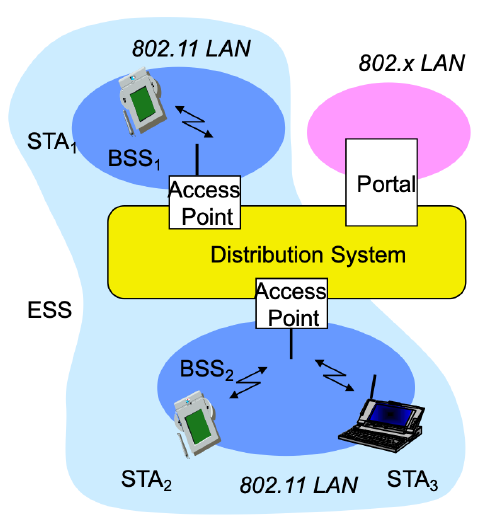
\includegraphics[scale=0.5]{images/9-wifi-terminology.png}
	\caption{WiFi System}%
	\label{fig:wifi-terminology}
\end{figure}

\begin{figure}[h]
	\centering
	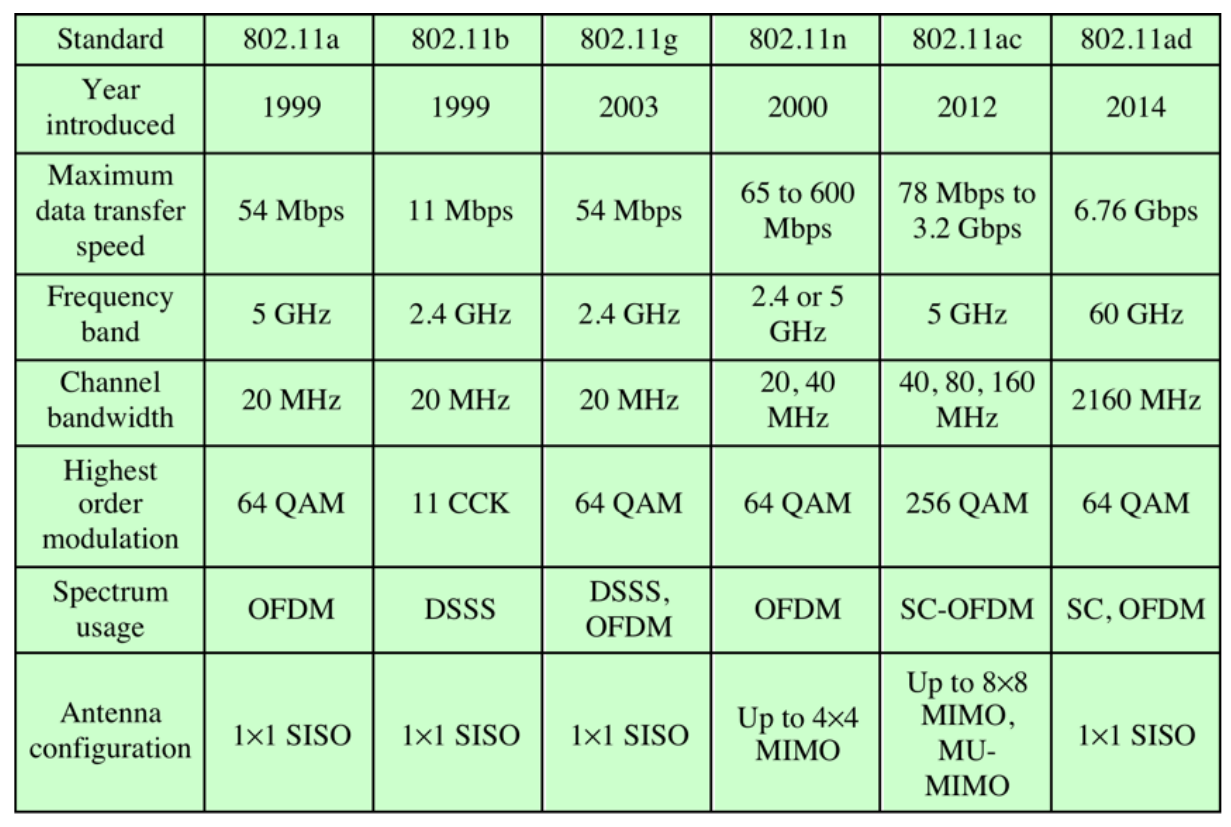
\includegraphics[scale=0.4]{images/9-wifi-versions.png}
	\caption{WiFi Standard Versions}%
	\label{fig:wifi-versions}
\end{figure}

\paragraph{Carrier-Sense Multiple Access with Collision Avoidance CSMA/CA}
Medium access control mechanism.
Part of the \textit{Distributed Coordination Function DCF}.
\begin{enumerate}
	\item \textit{Carrier sense} --- monitor medium to check if it is idle
	\item \textit{Collision avoidance} --- if another node sends, wait for a randomised \textit{backoff period}, then listen again
	\item \textit{Transmit} --- send entire frame, wait for ACK, if no ACK then backoff and wait
\end{enumerate}

\paragraph{Hidden terminal problem}
Occurs if a node B can communicate with two nodes A, C that cannot communicate with each other.
That is, if they both tried to send data to B they would individually sense the medium to be idle, but then they would clash at B anyway.
See \autoref{fig:hidden-terminal}.

The solution is to send a \textit{Request-to-Send RTS} message before transmitting a frame and wait for all nodes to reply with a \textit{Clear-to-Send CTS}.
Now when A sends a RTS even though C does not receive it, C still receives the CTS from B and will thus back off.
\\
This feature is optional in IEEE 802.11!

\begin{figure}[h]
	\centering
	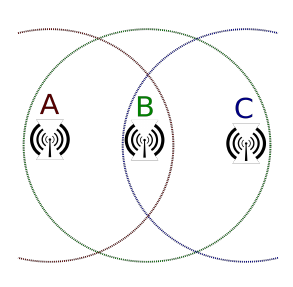
\includegraphics[scale=0.6]{images/9-hidden-terminal.png}
	\caption{Hidden Terminal Problem}%
	\label{fig:hidden-terminal}
\end{figure}

\paragraph{Frame types}
Data frames (user traffic), control frames (ACK, RTS/CTS), management frames (beacon\footnote{Contains basic information about the network, e.g. SSID, FH parameters, DSSS parameters, other supported options.}, association request, deauthentication).


\subsection{Basic Manipulations}

\paragraph{Capturing all frames}
Easy --- just install any packet capture software (such as Wireshark) and set the wireless interface to ``promiscuous mode''.

\paragraph{Communication (un)fairness}
DCF is fair --- assuming all stations adhere to it!
However by modifying backoff parameters in the wireless driver one can behave selfishly to get a higher throughput.

\paragraph{Jamming} \mbox{} \\
\underline{Simple:} \\
(a) Trigger carrier sense of transmitter (prevent sending, less power). \\
(b) Mangle the frame at the receiver (prevent receiving, more power).

\underline{Selective:} \\
Listen, decode prefix of an incoming frame and based on recipient address decide whether to jam the remaining data portion of the frame.
One needs to be very fast!

\paragraph{Man-in-the-middle}
Clone real AP onto different channel
$\rightarrow$ get clients to sign up to yours (e.g. jam real AP, send a Channel Switch Announcement CSA)
$\rightarrow$ inspect/manipulate/forward frames to real AP
$\rightarrow$ profit.


\subsection{WiFi Security Standards}

\subsubsection*{Wired Equivalent Privacy WEP}

First WiFi security standard (1997), with the goal of making wireless as secure as wired networks.
Today fully broken.

\underline{Operation:}\\
Checksum: plaintext $P = (m, CRC(m))$ \\
Encryption: ciphertext $C = P \oplus RC4(IV, k)$ (stream cipher RC4 with shared key $k$, initialisation vector $IV$) \\
Transmit $(IV, C)$.

\underline{Problems:}
\begin{itemize}
	\item \textit{Confidentiality}:
	Keystream reuse allows recovery of plaintexts:
	$$ C_1 \oplus C_2 = (P_1 \oplus RC4(IV,k)) \oplus (P_2 \oplus RC4(IV,k)) = P_1 \oplus P_2 $$
	Since the IV has 24 bits, at a data rate of 5 Mbps it will repeat after $\approx$ half a day.
	Knowing one of the plaintexts is reasonable (common structures such as IP headers, packet injection from the internet, other redundancies).
	\item \textit{Integrity}: CRC-32 is not a cryptographic MAC.
	This allows controlled message modification, i.e. given a $(ciphertext, checksum)$ pair we can create another $(ciphertext', checksum')$ pair such that the checksum is valid for the decrypted $plaintext'$.
	\item \textit{Access control}: works as follows:
	\begin{enumerate}
		\item AP sends a plaintext challenge
		\item Station replies with WEP encryption of challenge (proving possession of the key)
		\item AP completes association request
	\end{enumerate}
	Through simple traffic capture an adversary can learn a valid plaintext/ciphertext pair.
	From that they can derive the keystream to later compute a valid response to a new challenge (since the station can chose the IV).
\end{itemize}
Since 2007, tools like aircrack-ng allow recovering WEP keys in a matter of minutes.
\\
Wrong idea during design: ``in-flight'' modification of packets may be hard, but don't forget the possibility of offline attacks!


\subsubsection*{WiFi Protected Access WPA / Temporal Key Integrity Protocol TKIP}

Designed as a transitional mechanism in 2003 and to be compatible to WEP devices (though in 2019 still $\approx$ 50\% of networks accept it\dots).

\underline{Idea:}\\
Prevent keystream reuse and use a cryptographic MAC, while staying compatible to WEP.\@
``Achieved'' by augmenting encryption with per-packet key mixing, RC4 keystream filtering, a new integrity mechanism (MICHAEL) and counters for replay protection (TSC).
This allows to keep the WEP mechanism in hardware but change the inputs given to it.

\underline{ChopChop attack:} (for WEP!) \\
Capture an encrypted WEP frame.
Remove the last data byte, guess it, re-compute checksum for the shorter packet, use AP as an oracle (must discard frames whose checksums fail).
Rinse and repeat to learn one data block after the other.
\\
For a detailed explanation see \href{https://www.aircrack-ng.org/doku.php?id=chopchoptheory}{this aircrack doc entry}.
\\
Since this is a stream cipher, knowing one plaintext/ciphertext pair also reveals a keystream.

A similar attack also works for WPA/TKIP since MIC(HAEL) is reversible and the AP reports failures.

\underline{Biased keystream:} \\
There exist statistical biases in a RC4 keystream.
With enough packets this can be used to recover the plaintext for one MIC key.
Computationally expensive, but shows that crypto can be attacked, too.

\underline{Summary:}\\
Difficult start (had to reuse WEP hardware).
Raised the bar (despite ugly fix), but attacked in 2009, 2014/2015.
Okayish transition mechanism.


\subsubsection*{WPA2}

Introduced in 2004.
Better encryption (AES-128) and integrity (CBC-MAC, using \textit{authenticate-then-encrypt}).
Better authentication with a 4-way handshake.

\underline{Handshake:}\\
Goal: Starting from a \textit{Pairwise Master Key PMK} (that is derived from a shared passphrase) provide mutual authentication and establish a session key (\textit{Pairwise Transient Key PTK}).
\\
Steps: exchange nonces (msg1,2), derive PTK using PMK + nonces + MAC addresses, authenticate exchange (msg3,4).
Note that in msg2+3 the \textit{Message Integrity Code MIC} is also transmitted (missing in \autoref{fig:wpa2-handshake}).
\\
Proven ``secure'' in 2005 (mutual authentication and password is not leaked).

\begin{figure}[h]
	\centering
	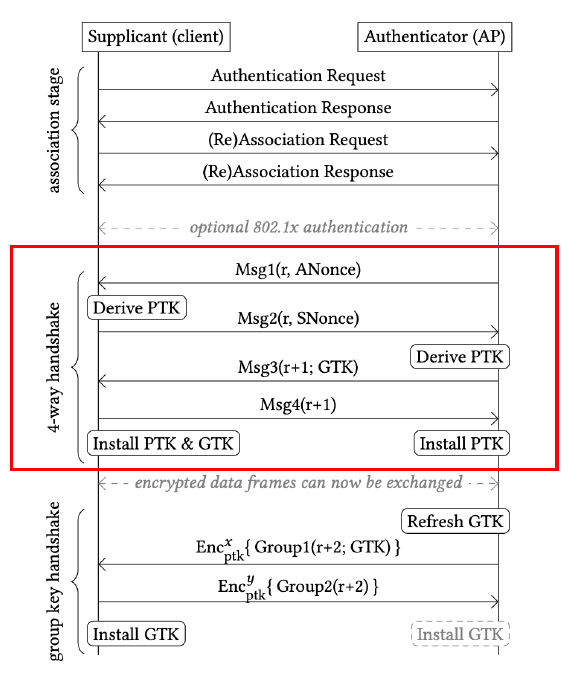
\includegraphics[scale=0.6]{images/9-wpa2-handshake.png}
	\caption{WPA2 Handshake}%
	\label{fig:wpa2-handshake}
\end{figure}

\underline{Dictionary attack}: \\
An adversary can capture the ANonce, SNonce and MIC.\@ \textit{If} the user chose a weak passphrase, then by brute force an attacker can try different passphrases, compute different PTKs and thus different MICs and compare the result to the captured MIC.\@

\href{https://www.krackattacks.com/}{\underline{Key Reinstallation Attack (KRACK)} (2017):} \\
Goal: force a keystream reuse.
\\
Observations: AP may retransmit msg3 if no ACK.\@ Each time, client reinstalls the \textit{same} PTK, and in the process it resets some counters.
This resulting in the same keystream being reused.
\\
Approach: Replay msg3.

\underline{Summary:}\\
Solid cryptography/encryption, weakness in handshake.
Proven properties hold, but model does not capture \textit{when} a key is installed.
Can be patched (and re-attacked).


\subsubsection*{WPA3}

Introduced in 2018.
Updated cryptography (AES-128/256 encryption, SHA-384 HMAC integrity), new handshake (based on the Dragonfly Key Exchange (\href{https://tools.ietf.org/html/rfc7664}{RFC 7664})).

\underline{Handshake improvements:}\\
Turns a low-entropy password into a high-entropy key, thus allowing for shorter passwords.
Has forward secrecy.

\href{https://wpa3.mathyvanhoef.com/}{\underline{Dragonblood} (2020):}\\
Transition mode allows downgrade to WPA2.
\\
Timing attack: execution time of turning the password into a group element at the start of the handshake depends on the password (i.e.\ a side-channel attack, though only for bad curves).

